\subsection{Méthode itérative}
Une autre approche souvent utilisée pour résoudre de grands systèmes d'équations linéaires creux consiste à utiliser des méthodes de résolution itérative~\cite{Saad96IMSLS}.
%
On appelle méthode itérative une méthode qui permet de résoudre un problème en partant d'une solution initiale $x_0$ et qui à chaque itération donne une nouvelle solution $x_i$.
%
Cette nouvelle solution $x_i$ étant plus proche de la solution exacte du problème que la solution précédente $x_{i-1}$.
%
La méthode s'arrête lorsque $x_i$ est suffisamment proche de la solution exacte selon un critère de convergence choisi.
%
Parmi ces méthodes nous pouvons citer la méthode Jacobi, Gauss-Seidel ou encore SOR, ce sont des méthodes itératives dites stationnaires.
%
Mais ces méthodes ne sont pas génériques, leur convergence dépend de certaines propriétés de la matrice.
%
Dans de nombreux cas concret, ces méthodes ne convergent pas rapidement si elles sont utilisées telles quelles.


La méthode du gradient conjugué est une méthode qui s'applique seulement à des matrices carrées symétriques définies positives.
%
Cette méthode permet de converger en au plus $n$ itérations avec $n$ la dimension de la matrice.
%
Mais avec un bon préconditionnement, on obtient rapidement une solution très proche de la solution exacte.
%
Puis cette méthode a été étendue aux matrices non-symétriques sous le nom du gradient biconjugué.
%
Le gradient biconjugué est une méthode par projection dans un espace de Krylov.
%
Le GMRES est aussi une méthode de Krylov et il fonctionne avec n'importe quelle matrice inversible.
%
Chaque itération du GMRES (Algo.~\ref{algo:gmres}) est composé d'un produit matrice vecteur creux (SpMV\footnote{Sparse Matrix Vector multiply}) ainsi que de plusieurs produits scalaires (DOT).

\begin{algorithm}
  \caption{GMRES avec une orthogonalisation Householder, nous avons surligné le produit matrice-vecteur creux ainsi que les produits scalaires.}
  \label{algo:gmres}
  \KwData{$m$ : Le nombre maximum d'itérations du GMRES}
  $r_0 := b - Ax_0$ \\
  $\beta := ||r_0||_2$ \\
  $v_1 := r_0/\beta$ \\
  Définir la $(m + 1)$x$m$ matrice $\overset{-}{H}_m = \{h_{ij}\}_{1 \leq i \leq m+1, 1 \leq j \leq m}$.  \\
  $\overset{-}{H}_m = 0$ \\
  \For{$j=1$ to $m$} {
    \tikz[baseline]{\node[fill=red!20,anchor=base]{$w_j := A * b$};}\\
    \For{\tikz[baseline]{\node[fill=blue!20,anchor=base]{$i=1$ {\bf à} $j$};}} {
      \tikz[baseline]{\node[fill=blue!20,anchor=base]{$h_{ij} := (w_j, v_i)$};} \\
      \tikz[baseline]{\node[fill=blue!20,anchor=base]{$w_j := w_j - h_{ij}v_i$};} \\
    }
    $h_{j+1,j} := ||w_j||_2$ \\
    \If{$h_{j+1,j} = 0$} {
      $m := j$ \\
      \textbf{break} \\
    }
    $v_{j+1} := w_j/h_{j+1,j}$ \\
  }
  Calculer $y_m$ le minimiseur de $||\beta{}e_1 - \overset{-}{H}_my||_2$ et $x_m := x_0 + V_my_m$
\end{algorithm}

La convergence (i.e. nombre d'itérations pour atteindre une précision donnée) des méthodes itératives dépend du nombre de conditionnement de la matrice $||A||_p.||A^{-1}||_p$ où $||A||_p$ est une norme multiplicative.
%
Plus ce nombre est grand, plus le nombre d'itérations est grand.
%
Comme les matrices utilisées dans la simulation de réservoir ne sont pas bien conditionnées, l'algorithme du GMRES ne converge qu'après beaucoup d'itérations.
%
Dans ce cas, nous pouvons préconditionner la matrice pour faire en sorte que le GMRES converge avec moins d'itérations.
%
Il faut choisir une matrice $M^{-1}$ tel que $M^{-1}A$ soit mieux conditionnées que $A$ (i.e. $||M^{-1}A||_p.||A^{-1}M||_p < ||A||_p.||A^{-1}||_p$).
%
Un cas idéal serait d'avoir $M=A$, dans ce cas là on obtient la matrice identité qui se trouve être très bien conditionnée.
%
Or, calculer $A^{-1}$ est très coûteux, à la fois en termes de calcul que de mémoire.



La factorisation LU permet de calculer directement $x=U^{-1}.L^{-1}.b=A^{-1}b$ mais comme nous l'avons vu, cette opération est très cher en calculs et en mémoire.
%
Néanmoins, une factorisation approchée de $A$, telle que $||A-LU||$ est relativement petite, peut jouer le rôle de préconditionneur dans une méthode de Krylov.
%
Ainsi, les factorisations ILU\footnote{Incomplete LU}\cite{Saad96IMSLS} sont des choix très populaires de préconditionneurs algébriques.
%
Les principales techniques de factorisation ILU visent à calculer une factorisation LU qui ne tient pas compte de certains coefficients de remplissage dans la matrice afin de limiter le coût tout en essayant de minimiser $||A-LU||$.
%
En effet, au cours de la factorisation, de nombreux termes de remplissage apparaîtront et l'espace mémoire nécessaire au stockage de ces nouveaux termes deviendrait gigantesque.
%
Mais nous ne sommes pas obligés de connaître parfaitement $A^{-1}$ pour obtenir un bon préconditionnement.
%
La méthode par précondionnement ILU est composée de deux opérations, la première correspond à la {\em factorisation} de la matrice en deux sous matrices, elle est faite juste avant le GMRES.
%
La deuxième correspond à la {\em résolution triangulaire} effectuée avec les deux sous matrices, elle est effectuée à chaque itération du GMRES.
%
Pour maintenir un espace mémoire raisonnable, on peut choisir de limiter le niveau de remplissage, les deux algorithmes les plus fréquemment utilisées sont :
\begin{itemize}
  \item Soit en fixant une valeur seuil à partir de laquelle le remplissage est accepté, il s'agit de l'algorithme ILUt;
  \item Soit en choisissant un niveau d'interaction maximal entre les lignes de la matrice, il s'agit de l'algorithme ILU(k) (Fig.~\ref{fig:iluk_filling}).
\end{itemize}

%   (-_-)   %
\begin{figure}[!h]
  \centering
  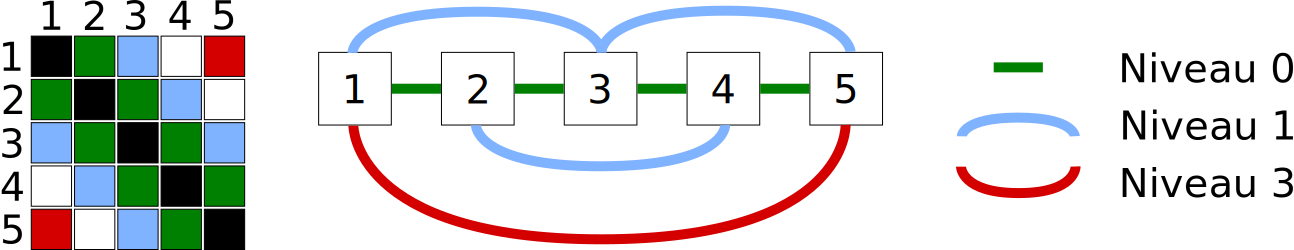
\includegraphics[width=\textwidth]{iluk_filling}
  \caption{Remplissage d'une matrice lors d'une factorisation ILU(k). Avec $k=2$ nous obtenons déjà le plus haut niveau de remplissage.}
  \label{fig:iluk_filling}
\end{figure}

La factorisation ILU(k) peut être faite en deux étapes :
\begin{itemize}
  \item une factorisation symbolique pour connaître le motif de non-zéros de la matrice;
  \item puis la factorisation réelle en utilisant ce motif.
\end{itemize}
%
La factorisation symbolique (Algo.~\ref{algo:iluk_symbolic}) va utiliser le graphe d'adjacence de la matrice.
%
S'il existe un chemin entre deux noeuds d'indices $i$ et $j$ tel que tous les indices du chemin soient inférieurs au minimum entre $i$ et $j$, alors une arête entre les noeuds $i$ et $j$ apparaîtra.
%
La longueur de ce chemin déterminera le niveau de remplissage.
%
Par exemple, sur la figure~\ref{fig:iluk_filling}, le noeud d'indice ``5'' aura une relation de niveau 2 avec le noeud d'indice ``4'' car le chemin 4-3-2-5 existe et les indices ``3'' et ``2'' sont inférieurs à ``4'' et ``5''.

%   (-_-)   %
\begin{figure}[!h]
  \centering
  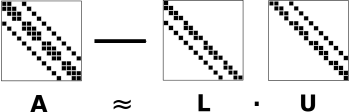
\includegraphics[width=\textwidth]{ilu0}
  \caption{Exemple de motif obtenu par une factorisation ILU(0), il n'y a pas de remplissage.}
  \label{fig:ilu0}
\end{figure}


\begin{algorithm}
  \label{algo:iluk_symbolic}
  \KwData{$A$ : La matrice à factoriser.\\
    $k$ : le niveau maximal de remplissage.}
  \For{chaque entrée $A_{ij}$ de $A$} {
    \If{$A_{ij} == 0$} { lev($A_{ij}$) := 0 }
    \If{$A_{ij} != 0$} { lev($A_{ij}$) := k+1 }
  }
  \For{$k=1$ {\bf à} $n-1$} {
    \For{$i=k+1$ {\bf à} $n$} {
      \If{lev($A_{ik}$) <= $k$} {
        \For{$j=k+1$ {\bf à} $n$} {
          lev($A_{ij}$) = min(lev($A_{ij}$), lev($A_{ik}$)+lev($A_{kj}$)+1) \\
          \If{lev($A_{ij}$) <= $k$} {
            on ajoute $A_{ij}$ au motif de non-zéro de la matrice.\\
          }
        }
      }
    }
  }
  \caption{Factorisation symbolique ILU(k)}
\end{algorithm}


L'algorithme ILUt a l'inconvénient d'avoir un motif de remplissage qui dépend des coefficients de la matrice.
%
Nous ne pouvons donc pas prévoir à l'avance l'espace nécessaire au stockage des matrices L et U et le stockage de ces matrices devient complexe.
%
Par contre, l'algorithme ILU(k) permet de connaître en avance le motif de remplissage de la matrice (Fig.~\ref{fig:iluk_filling}).
%
Il est donc possible de connaître la structure des matrices L et U à l'avance.
%
Pour la simulation de réservoir, nous utilisons l'algorithme ILU(k).
%
L'algorithme~\ref{algo:gmres_precond} représente un GMRES préconditionné avec une méthode ILU.


\begin{algorithm}
  \caption{GMRES préconditionné par une méthode ILU. Les parties surlignées correspondent au préconditionnement.}
  \label{algo:gmres_precond}
  \KwData{$m$ : Le nombre maximum d'itérations du GMRES}
  \tikz[baseline]{\node[fill=red!20,anchor=base]{$M =$ Factorisation\_ILU($A$)};} \\
  $r_0 := b - Ax_0$ \\
  $\beta := ||r_0||_2$ \\
  $v_1 := r_0/\beta$ \\
  Définir la $(m + 1)$x$m$ matrice $\overset{-}{H}_m = \{h_{ij}\}_{1 \leq i \leq m+1, 1 \leq j \leq m}$.  \\
  $\overset{-}{H}_m = 0$ \\
  \For{$j=1$ {\bf à} $m$} {
    \tikz[baseline]{\node[fill=yellow!20,anchor=base]{$temp :=$ Résolution\_Triangulaire($M, v_j$)};} \\
    $w_j := A * temp$\\
    \For{$i=1$ {\bf à} $j$} {
      $h_{ij} := (w_j, v_i)$ \\
      $w_j := w_j - h_{ij}v_i$ \\
    }
    $h_{j+1,j} := ||w_j||_2$ \\
    \If{$h_{j+1,j} = 0$} {
      $m := j$ \\
      \textbf{break} \\
    }
    $v_{j+1} := w_j/h_{j+1,j}$ \\
  }
  Calculer $y_m$ le minimiseur de $||\beta{}e_1 - \overset{-}{H}_my||_2$ et $x_m := x_0 + V_my_m$
\end{algorithm}
